\section{Green Roof Model (EcoRoof)}\label{green-roof-model-ecoroof}

\subsection{Overview}\label{overview-018}

The input object Material:RoofVegetation provides a model for green roofs (aka ecoroofs or vegetated roofs) that are becoming increasingly common for both new and retrofit buildings. There is widespread recognition and a growing literature of measured data that suggest green roofs can reduce building energy consumption. Currently, however, there are few design tools available to assist developers and architects in assessing the likely magnitude of energy savings associated with various implementation options (e.g., soil type/depth, irrigation options, plant type). As a result there is a significant need for a quantitative and physically-based building energy simulation tool that represents the effects of green roof constructions. Such a tool would facilitate more rapid spread of green roof technologies and make it possible to account for green roof benefits in state energy codes and related energy efficiency standards such as LEED.

In response to the need for green roof design tools a computational model of the heat transfer processes involved on a vegetated roof has been developed. This model accounts for:

\begin{itemize}
\item
  long wave and short wave radiative exchange within the plant canopy,
\item
  plant canopy effects on convective heat transfer,
\item
  evapotranspiration from the soil and plants, and
\item
  heat conduction (and storage) in the soil layer
\end{itemize}

The ability to track moisture-dependent thermal properties is not implemented yet due to stability issues in the CTF scheme, but is under development for use with the finite difference solution scheme made available in EnergyPlus starting in version 2.

As implemented in EnergyPlus the green roof module allows the user to specify ``ecoroof'' as the outer layer of a rooftop construction using a ``Material:RoofVegetation'' object. The user can then specify various aspects of the green roof construction including growing media depth, thermal properties, plant canopy density, plant height, stomatal conductance (ability to transpire moisture), and soil moisture conditions (including irrigation).

The model formulation includes the following:

\begin{itemize}
\item
  simplified moisture balance that allows precipitation, irrigation, and moisture transport between two soil layers (top and root zone).
\item
  soil and plant canopy energy balance based on the Army Corps of Engineers' FASST vegetation models (Frankenstein and Koenig), drawing heavily from BATS (Dickenson et al.) and SiB (Sellers et al.).
\item
  soil surface (T\(_{g}\)) and foliage (T\(_{f}\)) temperature equations are solved simultaneously each time step, inverting the CTF to extract heat flux information for the energy balance calculation.
\end{itemize}

The detailed energy balance analysis and resulting equations, being rather complicated, are summarized here. The interested reader is referred to the FASST documentation cited herein for the complete development. The end result is a set of two simultaneous equations for temperature---one for the soil surface and the other for the foliage.

\subsection{Green Roof Model Description}\label{green-roof-model-description}

As with a traditional roof, the energy balance of an green roof is dominated by radiative forcing from the sun. This solar radiation is balanced by sensible (convection) and latent (evaporative) heat flux from soil and plant surfaces combined with conduction of heat into the soil substrate. This energy balance is illustrated in Figure~\ref{fig:the-energy-balance-for-a-green-roof.}. The variables introduced in this figure are defined in the equations that follow.

\begin{figure}[hbtp] % fig 35
\centering
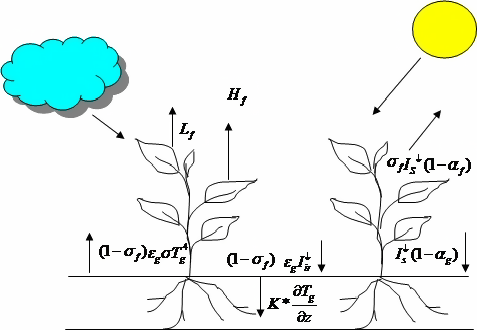
\includegraphics[width=0.9\textwidth, height=0.9\textheight, keepaspectratio=true]{media/image509.png}
\caption{The Energy Balance for a Green Roof. \protect \label{fig:the-energy-balance-for-a-green-roof.}}
\end{figure}

The energy budget analysis follows the Fast All Season Soil Strength (FASST) model developed by Frankenstein and Koenig for the US Army Corps of Engineers. FASST was developed, in part, to determine the ability of soils to support manned and unmanned vehicles and personnel movement. In order to accomplish this, however, FASST tracks the energy and moisture balance (including ice and snow) within a vegetated soil. It is a one-dimensional model that draws heavily from other plant canopy models including BATS (Dickinson et al.) and SiB (Sellers et al.). We have implemented FASST here with only a few modifications to adapt it for use with a relatively thin soil layer. The sign convention used assumes all heat fluxes are positive when energy is absorbed into the layer.

In the following discussion this energy budget is divided into a budget for the foliage layer (F\(_{f}\)) and a budget for the ground surface (F\(_{g-}\)). The various parameterizations for latent and sensible heat flux are described in some detail and then the equation set is reduced to the simultaneous solution of two equations involving the temperatures of the foliage and ground surface.

\subsubsection{Energy budget in the foliage layer}\label{energy-budget-in-the-foliage-layer}

The foliage energy balance is given by:

\begin{equation}
{F_f} = {\sigma_f}\left[ {{I_S}^ \downarrow (1 - {\alpha_f}) + {\varepsilon_f}{I_{ir}}^ \downarrow  - {\varepsilon_f}\sigma {T_f}^4} \right] + \frac{{{\sigma_f}{\varepsilon_g}{\varepsilon_f}\sigma }}{{{\varepsilon_1}}}\left( {{T_g}^4 - {T_f}^4} \right) + {H_f} + {L_f}
\end{equation}

Where $\sigma$\(_{f}\) is calculated as a function of Leaf-Area-Index (LAI):

\begin{equation}
\sigma_f = 0.9 - 0.7 \exp{-0.75 LAI }
\end{equation}

In addition to convective and sensible heat transfer this equation accounts for both the short and longwave radiation absorbed by the vegetation, including the effects of multiple reflections. The sensible and latent heat flux terms (H\(_{f}\) and L\(_{f-}\)) are somewhat complicated and therefore discussed in some detail below.

\paragraph{Sensible heat flux in the foliage layer}\label{sensible-heat-flux-in-the-foliage-layer}

The sensible heat transfer between the leaf surface and near-canopy air (H\(_{f}\)) is influenced by the temperature difference between them, wind speed, and Leaf Area Index (LAI). The Leaf Area Index is the dimensionless ratio of the projected leaf area for a unit ground area (Oke). In contrast fractional vegetative cover (s\(_{f}\)) is the ratio of shaded ground surface to total ground surface area. The sensible heat flux is given by:

\begin{equation}
{H_f} = (1.1*LAI{\rho_{af}}{C_{p,a}}{C_f}{W_{af}})*({T_{af}} - {T_f})
\end{equation}

In this equation the constant 1.1 accounts for heat transfer from the stems, twigs and limbs (Deardorff). The properties of air near the foliage are modeled using the average from the foliage and instrument conditions:

\begin{equation}
{\rho_{af}} = 0.5({\rho_a} + {\rho_f})
\end{equation}

where r\(_{a}\) is the density of air at the instrument height ~and r\(_{f}\) is the density of air at the leaf temperature. The air temperature within the foliage is estimated by:

\begin{equation}
{T_{af}} = (1 - {\sigma_f})({T_a}) + {\sigma_f}\left( {0.3{T_a} + 0.6{T_f} + 0.1{T_g}} \right)
\end{equation}

\emph{where, T\(_{a}\)} is the air temperature at the instrument height in Kelvin \emph{T\(_{f}\)}, is leaf temperature in Kelvin and \emph{T\(_{g}\)}, is the ground surface temperature in Kelvin. The foliage wind speed is estimated as:

\begin{equation}
{W_{af}} = 0.83{\sigma_f}W\sqrt {C_{hn}^f}  + (1 - {\sigma_f})W
\end{equation}

Here \emph{W} is the larger of 2.0 m/s or the actual wind speed above the canopy (Hughes et al.) and C\(^{f}\)\(_{hn}\) is the transfer coefficient at near-neutral atmospheric stability conditions:

\begin{equation}
C_{hn}^f = {K_v}^2 \cdot {\left( {\ln \left( {\frac{{{Z_a} - {Z_d}}}{{Z_o^f}}} \right)} \right)^{ - 2}}
\end{equation}

where \emph{K\(_{v}\),} is von Karmen's constant (0.4), Z\(_{a}\) is the instrument height, Z\(_{d}\) is the zero displacement height in meters (height above soil within which the wind speed is effectively zero), and Z\(^{f}\)\(_{o}\) is the foliage roughness length scale (m). The formulations for zero displacement height, roughness length are based on Balick et al.:

\begin{equation}
{Z_d} = 0.701Z_{_f}^{0.979}
\end{equation}

\begin{equation}
{Z_o} = 0.131Z_{_f}^{0.997}
\end{equation}

Finally, the bulk transfer coefficient as defined by Deardorff is given by:

\begin{equation}
{C_f} = 0.01*\left( {1 + \frac{{0.3(m/s)}}{{{W_{af}}(m/s)}}} \right)
\end{equation}

\paragraph{Latent heat flux in the foliage layer}\label{latent-heat-flux-in-the-foliage-layer}

The process of water loss through plant respiration is known as transpiration. It is controlled by the closing and opening of stomata - the intercellular openings between to epidermal (guard) cells (Gates). The resistance to the diffusion of water vapor from these spaces into the atmosphere is called stomatal resistance. It depends on factors such as light intensity, soil moisture content and vapor pressure difference between inside leaf and the outside atmosphere. It is measured in units of s/m and is formulated as:

\begin{equation}
{r_s} = \frac{{{r_{s,\min }}}}{{LAI}} \cdot {f_1} \cdot {f_2} \cdot {f_3}
\end{equation}

Here, r\(_{s,min}\) is the minimum stomatal resistance. The actual stomatal resistance at any time is proportional to this minimum resistance and inversely proportional to LAI. The stomatal resistance is further modified by fractional multiplying factors that relate to incoming solar radiation and atmospheric moisture. As found in Frankenstein and Koenig the inverses of the multiplying factors f\(_{1}\), f\(_{2}\), and f\(_{3}\) are given by:

\begin{equation}
\begin{array}{l}
   \frac{1}{f_1} = \min \left[ 1,\frac{{0.004*{I_s}^ \downarrow  + 0.005}}{{0.81*(0.004*{I_s}^ \downarrow  + 1)}} \right] \\
   \frac{1}{f_2} = \left\{ 
     \begin{array}{cl}
       0                                                                 & \text{when} \; \theta_r > \overline \theta \\
       \frac{ \overline \theta   - \theta_r }{ \theta_{max} - \theta_r } & \text{when} \; \theta_r \leq \overline \theta \leq \theta_{max}
     \end{array} \right. \\
   \frac{1}{f_3} = \exp \left[ - {g_d}({e_{f,sat}} - {e_a} \right]
\end{array}
\end{equation}

Here, Q\(_{r}\), is the residual moisture content (defined as the amount of moisture in soil when plants begin to wilt), Q\(_{max}\) is the maximum moisture content (defined as the maximum amount of moisture a particular type of soil can hold and above which run off occurs), and \(\overline \Theta\) ~is the average soil moisture in the root zone. The residual moisture content is typically around 0.01 m\(^{3}\)/m\(^{3}\) (Frankenstein and Koenig). The maximum moisture content depends upon the soil, but generally varies from 0.3 to 0.6 m\(^{3}\)/m\(^{3}\) (Guymon et al.). In the expression for f\(_{3}\), g\(_{d}\) is a plant specific characteristic that is only non-zero for trees, e\(_{f,sat}\) is the saturated vapor pressure at the leaf temperature, and e\(_{a}\) is the air vapor pressure.

Resistance to moisture exchange offered by the boundary layer formed on the leaf surface is known as aerodynamic resistance. It is measured in units of (s/m) and is influenced by wind speed, surface roughness and stability of the atmosphere (Oke). It is formulated as:

\begin{equation}
{r_a} = \frac{1}{{{c_f}{W_{af}}}}
\end{equation}

The combined effect of aerodynamic and stomatal resistances to vapor diffusion is integrated into a foliage surface wetness factor:

\begin{equation}
r'' = \frac{{{r_a}}}{{{r_a} + {r_s}}}
\end{equation}

This surface wetness factor is simply a ratio of the aerodynamic resistance to the total resistance. When the aerodynamic resistance is small the wetness factor approaches zero (leaf surfaces remain dry as surface moisture is readily evaporated). As the aerodynamic resistance increases in importance relative to stomatal resistance the wetness factor approaches 1.0 (moisture readily travels to the leaf surfaces, but is not easily evaporated).

The latent heat flux is then given by:

\begin{equation}
{L_f} = {l_f} * LAI{\rho_{af}}{C_f}{W_{af}}{r^``}\left( {{q_{af}} - {q_{f,sat}}} \right)
\end{equation}

Here \emph{l\(_{f}\)} , is the latent heat of vaporization (J/kg), q\(_{f,sat}\) is the saturation mixing ratio at the leaf surface temperature, and q\(_{af}\) is the mixing ratio of the air within the canopy. As developed in Frankenstein and Koenig the mixing ratio within the canopy can be determined from:

\begin{equation}
{q_{af}} = \left[ {\frac{{\left( {1 - {\sigma_f}} \right){q_a} + {\sigma_f}\left( {0.3{q_a} + 0.6{q_{f,sat}}{r^``} + 0.1{q_{f,sat}}{M_g}} \right)}}{{1 - {\sigma_f}\left[ {0.6\left( {1 - {r^``}} \right) + 0.1\left( {1 - {M_g}} \right)} \right]}}} \right]
\end{equation}

where the factor \emph{M\(_{g}\)} ~(ranging from 0 to 1) is the ratio of volumetric moisture content to the porosity of the soil (Koenig). The latent heat of vaporization (\emph{l\(_{f}\)}) is the amount of energy required to convert a unit mass of water to vapor. It is measured in units of J/kg and is inversely proportional to the temperature. From Henderson-Sellers it is estimated as:

\begin{equation}
{l_f} = 1.91846*{10^6}{\left[ {\frac{{{T_f}}}{{{T_f} - 33.91}}} \right]^2}
\end{equation}

\subsubsection{Soil Energy budget}\label{soil-energy-budget}

The energy budget at the soil surface is mainly influenced by the soil thermal properties, the amount of foliage coverage (s\(_{f}\)) and the amount of moisture in the soil. If the soil surface is densely covered the diurnal range of surface temperature is small. In the soil energy budget the heat released or gained due to phase changes of soil water, precipitation heat flux and heat flux due to vertical transport of water in the soil are ignored. Future refinements to this model will incorporate these phenomena. The sign convention followed here is the same as above (heat flux into the soil is positive). The overall energy balance at the soil surface (as given in Frankenstein and Koenig) is:

\begin{equation}
{F_g} = (1 - {\sigma_f})\left[ {I_s^ \downarrow (1 - {\alpha_g}) + {\varepsilon_g}I_{ir}^ \downarrow  - {\varepsilon_g}T_g^4} \right] - \frac{{{\sigma_f}{\varepsilon_g}{\varepsilon_f}\sigma }}{{{\varepsilon_1}}}\left( {T_g^4 - T_f^4} \right) + {H_g} + {L_g} + K*\frac{{\partial {T_g}}}{{\partial z}}
\end{equation}

As with the energy equation for the foliage this equation represents sensible heat flux (H\(_{g}\)), latent heat flux (L\(_{g}\)) and the multiple reflections associated with long and short wave radiation. The final term on the right side gives the conduction of heat into the soil substrate.

\paragraph{Sensible heat flux in the soil layer}\label{sensible-heat-flux-in-the-soil-layer}

Sensible heat flux between the soil surface and air in its vicinity is dependent on the temperature difference between them and the wind speed within the canopy. It is given as

\begin{equation}
{H_g} = {\rho_{ag}}{C_{p,a}}C_h^g{W_{af}}({T_{af}} - {T_g})
\end{equation}

where \(C_h^g\) ~is the bulk transfer coefficient and r\(_{ag}\) is the density of air near the soil surface (kg/m\(^{3}\)) given by:

\begin{equation}
{p_{ag}} = \frac{{{p_a} + {p_g}}}{2}
\end{equation}

Here r\(_{g}\) is the density of air at the ground surface temperature

The bulk transfer coefficient is given as the linear combination of bulk transfer coefficient near ground (C\(^{f}\)\(_{hn}\)) and near foliage-atmosphere interface (C\(^{g}\)\(_{hn}\)) multiplied by the stability factor (G\(_{h}\)) and is formulated as:

\begin{equation}
C_h^g = {\Gamma_k}\left[ {\left( {1 - {\sigma_f}} \right)C_{hn}^g + {\sigma_f}C_{hn}^f} \right]
\end{equation}

The ground and foliage bulk transfer coefficients, in turn, are given by:

\begin{equation}
C_{hn}^g = r_{ch}^{ - 1}{\left[ {\frac{{{K_v}}}{{\ln \left( \frac{Z_a}{Z_o^g} \right)}}} \right]^2}
\end{equation}

And

\begin{equation}
C_{hn}^f = {\left[ {\frac{{K_v}}{{\ln \left( \frac{{Z_a} - {Z_d}}{Z_o^f} \right)}}} \right]^2}
\end{equation}

where\(Z_o^g\) ~and \(Z_o^f\) ~are the ground and foliage roughness lengths,~ r\(_{ch}\) is turbulent Schmidt number (0.63), and K\(_{v}\) is the von Karman constant (0.4).

The condition of the atmosphere (G\(_{h}\)) is determined as stable or unstable based on the sign of the bulk Richardson number:

\begin{equation}
{R_{ib}} = \frac{{2g{Z_a}\left( {{T_{af}} - {T_g}} \right)}}{{\left( {{T_{af}} + {T_g}} \right)W_{af}^2}}
\end{equation}

The atmospheric stability factor is then given by Businger and Lumley and Panofsky as:

\begin{equation}
\Gamma_h = \left\{ 
    \begin{array}{cl}
      \frac{1.0}{\left( 1.0 - 16.0 R_{ib} \right)^{0.5}} & \text{for} \; R_{ib} < 0 \\
      \frac{1.0}{\left( 1.0 - 5.0  R_{ib} \right)      } & \text{for} \; R_{ib} > 0
    \end{array}
  \right.
\end{equation}

\paragraph{Latent heat flux in the soil layer}\label{latent-heat-flux-in-the-soil-layer}

Removal of water vapor from the soil surface depends on the difference between the mixing ratio of the soil surface and air and the wind speed within the canopy. The resulting latent heat flux is then given by:

\begin{equation}
{L_R} = C_e^g{l_g}{W_{af}}{\rho_{ag}}\left( {{q_{af}} - {q_g}} \right)
\end{equation}

Here\(C_e^g\) is the bulk transfer coefficient, l\(_{g}\) is the latent heat of vaporization at the ground surface temperature, q\(_{af}\) is the mixing ratio at the foliage-atmosphere interface, and q\(_{f}\) is the mixing ratio at the ground surface, given by:

\begin{equation}
{q_g} = {M_g}{q_{g,sat}} + \left( {1 - {M_g}} \right){q_{af}}
\end{equation}

The bulk transfer coefficient for latent heat exchange is analogous to that for sensible heat exchange and is given by:

\begin{equation}
C_e^g = {\Gamma_e}\left[ {\left( {1 - {\sigma_f}} \right)C_{en}^g + {\sigma_f}C_{hn}^f} \right]
\end{equation}

where \(C_{en}^g\) is the near ground bulk transfer coefficient for Latent heat flux and G\(_{e}\) is the latent heat exchange stability correction factor (assumed to be the same as G\(_{h}\)).

\subsection{Linearization}\label{linearization}

In order to solve the foliage and soil heat budget equations, the 4\(^{th}\) order terms T\(_{f}\)\(^{4}\) and T\(_{g}\)\(^{4}\) ~and mixing ratio terms q\(_{g,sat}\) and q\(_{f,sat}\) are linearized as given by Deardorff:

\begin{equation}
{\left[ {T_f^{\left( {n + 1} \right)}} \right]^4} = {\left[ {T_f^n} \right]^4} + 4{\left[ {T_f^n} \right]^3}\left[ {T_f^{n + 1} - T_f^n} \right]
\end{equation}

\begin{equation}
{\left[ {T_g^{\left( {n + 1} \right)}} \right]^4} = {\left[ {T_g^n} \right]^4} + 4{\left[ {T_g^n} \right]^3}\left[ {T_g^{n + 1} - T_g^n} \right]
\end{equation}

Here T\(_{f}\)\(^{n+1}\) and T\(_{g}\)\(^{n+1}\) are the current time step leaf and ground surface temperatures in Kelvin. T\(_{f}\)\(^{n}\) and T\(_{g}\)\(^{n}\) are the corresponding temperatures at the previous time step.

The saturation mixing ratio at the ground and leaf surface temperatures are given as:

\begin{equation}
{q_{g,sat}}\left( {T_g^{n + 1}} \right) = {q_{sat}}\left( {T_g^n} \right) + {\left( {\frac{{\partial {q_{sat}}}}{{\partial T}}} \right)_{T_g^n}} * \left( {T_g^{n + 1} - T_g^n} \right)
\end{equation}

\begin{equation}
{q_{f,sat}}\left( {T_f^{n + 1}} \right) = {q_{sat}}\left( {T_f^n} \right) + {\left( {\frac{{\partial {q_{sat}}}}{{\partial T}}} \right)_{T_f^n}} * \left( {T_f^{n + 1} - T_f^n} \right)
\end{equation}

where q\(_{sat}\)(T\(_{g}\)\(^{n}\)) is the saturation mixing ratio at the previous time step and is formulated as given in Garratt:

\begin{equation}
{q_{sat}}\left( {T_g^n} \right) = \frac{{0.622{e^ * }\left( {T_g^n} \right)}}{{P - {e^ * }\left( {T_g^n} \right)}}
\end{equation}

Here the saturation vapor pressure e* (Pa) is evaluated at the ground temperature from the previous time step (T\(_{g}\)\(^{n}\)) as:

\begin{equation}
{e^*} = 611.2\exp \left[ {17.67\left( {\frac{{T_g^n - 273.15}}{{T_g^n - 29.65}}} \right)} \right]
\end{equation}

The derivative of saturation mixing ratio at the previous time step is given by:

\begin{equation}
\frac{{d{q^ * }}}{{dT_g^n}} = \left[ {\frac{{0.622 * P}}{{{{\left( {P - 0.378 * {e^ * }} \right)}^2}}}} \right]\left( {\frac{{d{e^ * }}}{{dT_g^n}}} \right)
\end{equation}

Here, the derivative of the saturation vapor pressure can be calculated from the Clausius-Clapeyron equation:

\begin{equation}
\frac{{d{e^ * }}}{{dT_g^n}} = \frac{{{l_g} * {e^ * }\left( {T_g^n} \right)}}{{\left( {{R_v} * {{\left( {T_g^n} \right)}^2}} \right)}}
\end{equation}

Where R\(_{v}\) is the gas constant for water vapor and l\(_{g}\) is the latent heat of vaporization at the soil surface temperature.

The corresponding saturation mixing ratio relations for the leaf surfaces can be obtained by replacing T\(_{g}\) with T\(_{f}\) in the above relations.

\subsection{Final Equations}\label{final-equations}

After linearization the final equations are of the form:

\begin{equation}
C_1^f + C_2^f{T_g} + C_3^f{T_f} = 0
\end{equation}

\begin{equation}
C_1^g + C_2^g{T_g} + C_3^g{T_f} = 0
\end{equation}

The coefficients in these equations result from the direct combination of the equations from the above development. The interested reader is directed to the papers by Frankenstein and Koenig for the complete and somewhat complicated expressions.

This final set of equations is then solved simultaneously to obtain T\emph{\(_{g}\)} and T\emph{\(_{f}\)} . One key difference in our implementation of the FASST algorithm is that the conduction terms in the equations for \(C_1^g\) and \(C_2^g\) ~are solved by inverting the Conduction Transfer Functions (CTF) within the EnergyPlus solution scheme.

\subsection{Green Roof Nomenclature}\label{green-roof-nomenclature}

C\(_{1}\), C\(_{2}\), C\(_{3}\)~~~ = ~~~~~~~~~ coefficients in linearized temperature equations

\emph{C\(_{e}\)\(^{g}\)~~~~~~~~~~~~~ = ~~~~~~~~~} latent heat flux bulk transfer coefficient at ground layer

\emph{C\(_{f}\)~~ ~~~~~~~~~~~} = ~~~~~~~~~ bulk heat transfer coefficient

C\(_{h}\)\(^{g}\)~~~~~~~~~~~~~ = ~~~~~~~~~ sensible heat flux bulk transfer coefficient at ground layer

C\(_{hn}\)\(^{f}\) ~~~~~~~~~~~ = ~~~~~~~~~ near-neutral transfer coefficient at foliage layer

C\(_{hn}\)\(^{g}\) = ~~~~~~~~~ near-neutral transfer coefficient at ground layer

C\(_{p,a}\)~~~~~~~~~~~~ = ~~~~~~~~~ specific heat of air at constant pressure (1005.6 J/kg k)

e\(^{*}\)~~~~~~~~~~~~~~~ = ~~~~~~~~~ saturation vapor pressure (Pa)

f\(_{1}\)~~~~~~~~~~~~~~~ = ~~~~~~~~~ multiplying factor for radiation effect on stomatal resistance

f\(_{2}\)~~~~~~~~~~~~~~~ = ~~~~~~~~~ multiplying factor for moisture effect on stomatal resistance

f\(_{3}\)~~~~~~~~~~~~~~~ = ~~~~~~~~~ additional multiplying factor for stomatal resistance

F\(_{f}\)~~~~~~~~~~~~~~~ = ~~~~~~~~~ net heat flux to foliage layer (W/m\(^{2}\))

F\(_{g}\)~~~~~~~~~~~~~~ = ~~~~~~~~~ net heat flux to ground surface (W/m\(^{2}\))

g\(_{d}\)~~~~~~~~~~~~~~ = ~~~~~~~~~ plant specific characteristic related to stomatal resistance

H \emph{\(_{f}\)} ~~~~~~~~~~~~~ = ~~~~~~~~~ foliage sensible heat flux (W/m\(^{2}\))

H\(_{g}\)~~~~~~~~~~~~~~ = ~~~~~~~~~ ground sensible heat flux (W/m\(^{2}\))

\(I_s^ \downarrow\) ~~~~~~~~~~~ = ~~~~~~~~~ total incoming short wave radiation (W/m\(^{2}\))

\(I_{i\gamma }^ \downarrow\) ~~~~~~~~~~~~ = ~~~~~~~~~ total incoming longwave radiation (W/m\(^{2}\))

K\(_{v}\)~~~~~~~~~~~~~~ = ~~~~~~~~~ von Karmen constant (0.4)

l\(_{f}\)~~~~~~~~~~~~~~~~ = ~~~~~~~~~ latent heat of vaporization at foliage temperature (J/kg)

l\(_{g}\)~~~~~~~~~~~~~~~ = ~~~~~~~~~ latent heat of vaporization at ground temperature (J/kg)

L\emph{\(_{f}\)}~ ~~~~~~~~~~~~~ = ~~~~~~~~~ foliage latent heat flux (W/m\(^{2}\))

L\(_{g}\)~~~~~~~~~~~~~~ = ~~~~~~~~~ ground latent heat flux (W/m\(^{2}\))

\emph{LAI}~ ~~~~~~~~~~ = ~~~~~~~~~ leaf area index (m\(^{2}\)/m\(^{2}\))

M\(_{g}\)~~~~~~~~~~~~~ = ~~~~~~~~~ moisture saturation factor

q\(_{a}\)~~~~~~~~~~~~~~ = ~~~~~~~~~ mixing ratio for air

q\(_{af}\)~~~~~~~~~~~~~~ = ~~~~~~~~~ mixing ratio for air within foliage canopy

q\(_{f,sat}\)~~~~~~~~~~~~ = ~~~~~~~~~ saturation mixing ratio at foliage temperature

q\(_{g,sat}\)~~~~~~~~~~~ = ~~~~~~~~~ saturation mixing ratio at ground temperature

r\(_{a}\)~~~~~~~~~~~~~~~ = ~~~~~~~~~ aerodynamic resistance to transpiration (s/m)

r\(_{s}\)~~~~~~~~~~~~~~~ = ~~~~~~~~~ foliage leaf stomatal resistance (s/m)

r\(_{s,min}\)~~~~~~~~~~~ = ~~~~~~~~~ minimal leaf stomatal resistance (s/m)

r''~~~~~~~~~~~~~~~ = ~~~~~~~~~ surface wetness factor

R\(_{ib}\)~~~~~~~~~~~~~ = ~~~~~~~~~ bulk Richardson number

R\(_{v}\)~~~~~~~~~~~~~~ = ~~~~~~~~~ gas constant for water vapor (461.53 J/kgK)

\emph{T\(_{a}\)} = ~~~~~~~~~ the air temperature at the instrument height (Kelvin)

T\(_{af}\) ~ ~~~~~~~~~ = ~~~~~~~~~ air temperature with in the canopy (Kelvin)

T\emph{\(_{f}\)}~~ ~~~~~~~~~~~ = ~~~~~~~~~ leaf temperature (Kelvin)

T\(_{g}\) ~~~~~~~~~~~~~~ = ~~~~~~~~~ ground surface temperature (Kelvin)

W~~~~~~~~~~~~~~ = ~~~~~~~~~ wind speed above canopy (m/s)

W\(_{af}\)~ ~~~~~~~~~~~ = ~~~~~~~~~ wind speed with in the canopy (m/s)

z~~~~~~~~~~~~~~~~ = ~~~~~~~~~ height or depth (m)

Z\(_{a}\)~~~~~~~~~~~~~~ = ~~~~~~~~~ instrument height (m)

Z\(_{d}\)~~~~~~~~~~~~~~ = ~~~~~~~~~ displacement height (m)

Z\(_{o}\)\(^{f}\)~~~~~~~~~~~~~~ = ~~~~~~~~~ foliage roughness length scale (m)

\subsubsection{Greek letters}\label{greek-letters-000}

\(\alpha\)\(_{f}\)~~~ ~~~~~~~~~~~ = ~~~~~~~~~ albedo (short wave reflectivity) of the canopy

\(\alpha\)\(_{g}\)~~~~~~~~~~~~~~ = ~~~~~~~~~ albedo (short wave reflectivity) of ground surface

\(\varepsilon\)\(_{1}\)~~~~~~~~~~~~~ = ~~~~~~~~~ \(\varepsilon\)\(_{g}\) + \(\varepsilon\)\(_{f}\)  - \(\varepsilon\)\(_{f}\)\(\varepsilon\)\(_{g}\)

\(\varepsilon\)\(_{f}\) ~~~~~~~~~~~ = ~~~~~~~~~ emissivity of canopy 

\(\varepsilon\)\(_{g}\) ~~~~~~~~~~~ = ~~~~~~~~~ emissivity of the ground surface

\(\Gamma\)\(_{h}\)~~~~~~~~~~~~~~~~~~~ = ~~~~~~~~~~~~~stability factor

\(\rho\)\(_{a}\)~ ~~~~~~~~~~~~ = ~~~~~~~~ density of air at instrument height (kg/m\(^{3}\))

\(\rho\)\(_{f}\)~ ~~~~~~~~~~~~~ = ~~~~~~~~ density of air at foliage temperature (kg/m\(^{3}\))

\(\rho\)\(_{f}\)~ ~~~~~~~~~~~~ = ~~~~~~~~ density of air at foliage temperature (kg/m\(^{3}\))

\(\rho\)\(_{g}\)~~~~~~~~~~~~~ = ~~~~~~~~ density of air at ground surface temperature (kg/m\(^{3}\))

\(\sigma\) ~ ~~~~~~~~~~~ = ~~~~~~~~~ the Stefan-Boltzmann constant (5.699*10\(^{8}\) W/m\(^{2}\) $^{\circ}$K\(^{4}\))

\(\sigma\)\(_f\) ~~~~~~~~~~~ ~~~~~~~~~~~ = ~~~~~~~~~ fractional vegetation coverage

\subsubsection{Subscripts and superscripts}\label{subscripts-and-superscripts-000}

a~~~~~~~~~~~~~~~ = ~~~~~~~~~ air

af~~~~~~~~~~~~~~ = ~~~~~~~~~ air within the foliage layer

e~~~~~~~~~~~~~~~ = ~~~~~~~~~ latent heat flux term

f~~~~~~~~~~~~~~~~ = ~~~~~~~~~ foliage surface

g~~~~~~~~~~~~~~~ = ~~~~~~~~~ ground surface

h~~~~~~~~~~~~~~~ = ~~~~~~~~~ sensible heat flux term

n~~~~~~~~~~~~~~~ = ~~~~~~~~~ current time step

n+1~~~~~~~~~~~~ = ~~~~~~~~~ future time step

ir~~~~~~~~~~~~~~~ = ~~~~~~~~~ infrared (or long-wave)

sat~~~~~~~~~~~~~ = ~~~~~~~~~ saturation value

S~~~~~~~~~~~~~~~ = ~~~~~~~~~ short-wave

\subsection{References}\label{references-025}

ASHRAE. 2005. 2005 ASHRAE Handbook -- Fundamentals. Chapter 16, Air flow Around Buildings, Atlanta: American Society of Heating Refrigerating and Air-Conditioning Engineers, Inc.

Balick, L. R., R. K. Scoggins, and L. E. Link. 1981. Inclusion of a simple vegetation layer in terrain temperature models for thermal IR signature prediction. IEEE Geoscience and Remote Sensing GE-19(3), pp.143-152.

Businger, J. A. 1966. In `Arctic Heat Budget and Atmospheric Circulation', Symposium Proceedings, pp.~305-332. The Rand Corporation.

Deardorff, J.W. 1978. ``Efficient Prediction of ground surface temperature and moisture with inclusion of a layer of vegetation'', Journal Geophysical Research, pp.~1889-1902.

Dickinson, R.E., A. Henderson-Sellers, P.J. Kennedy, and M.F. Wilson. 1986. Biosphere-Atmosphere Transfer Scheme (BATS) for the NCAR community climate model. NCAR Technical Note, TN-275+STR.

ECMWF. 2002. European Centre for Medium-Range Weather Forecasts, Integrated Forecast System. Documentation, CY25R1 (Operational implementation 9 April 2002). .

Frankenstein, S., and G. Koenig. 2004.FASST Vegetation Models. U. S. Army Engineer Research and Development Center, Cold regions Research and Engineering Laboratory, ERDC/CRREL Technical Report TR-04-25.

Frankenstein, S., and G. Koenig. 2004.Fast All-season Soil Strength (FASST). U.S. Army Engineer Research and Development Center, Cold regions Research and Engineering Laboratory, ERDC/CRREL Special Report SR-04-1.

Garratt, J.R. 1992. The Atmospheric Boundary Layer, Cambridge university press.

Gates, D.M. 1980. Biophysical Ecology. New York: Springer-Verlag

Guymon, G.L., R.L. Berg, and T.V. Hromadka. 1993. Mathematical Model of Frost Heave and Thaw Settlement in Pavements. U.S. Army Cold Regions Research and Engineering Laboratory, CRREL Report 93-2.

Henderson-Sellers, B. 1984. ``A New Formula for Latent Heat of Vaporization of water as function of temperature'', Quarterly Journal Royal Meteorological Society, 10 pp.~1186-1190.

Hughes, P.A., T.J.L. McComb, A.B. Rimmer, and K.E. Turver. 1993. ``A mathematical model for the prediction of temperature of man-made and natural surfaces'', International Journal of Remote Sensing 14 (7), pp.~1383-1412.

Koenig, G.G. 1994. Smart Weapons Operability Enhancement (SWOE) Joint Test and Evaluation (JT and E) Program: Final Report. Dr.~James P. Welch, Joint Test Director, SWOE JT and E, SWOE Report 94-10, Annex D.

Lumley, J. L. and Panofsky, H. A. 1964. `The structure of Atmospheric Turbulence'. Interscience Monographs and Texts in Physics and Astronomy, Vol. XII. Wiley, New York.

Oke, T.R. 1987. Boundary Layer Climates, University Press, Cambridge

Sellers, P.J., Y. Mintz, Y.C. Sud, and A. Dalcher. 1986. A simple biosphere model (SiB) for use within general circulation models. Journal of Atmospheric Science, 43 (6), pp.~505-532.
